% vim: set tw=78 sts=2 sw=2 ts=8 aw et ai:
\documentclass{soa.cs.pub.ro}

\usepackage{color}
\usepackage{alltt}
\usepackage{verbatim}
\usepackage{listings}
\usepackage[absolute,overlay]{textpos}

\title[Project Title Abbreviation]{Project Title}
\subtitle{Team Name}
\date{day month year}

\begin{document}

\frame{\titlepage}

\frame{\tableofcontents}

\section{Introducere}

\begin{frame}{Introducere}
  \begin{itemize}
    \item Mai importantă WLAN acoperirea decât performanța
    \item Performanța este lăsată în seama protocolului de la nivel fizic
    \item Multe device-uri, banda este împărțită
  \end{itemize}
\end{frame}

\begin{frame}{DenseAP}
  \begin{itemize}
    \item Multe AP-uri, cu puțini clienți
    \item Clienții nu trebuie modificați
    \pause
    \item Alegerea AP-ului este lăsată în seama rețelei, nu a clientului
    \item Sistem centralizat de asociere, care colectează informații de trafic de la AP-uri
  \end{itemize}
\end{frame}



\section{Boiling point}

\begin{frame}{Problem}
  \begin{columns}
    \pause
    \begin{column}[l]{0.45\textwidth}
      \begin{center}
        A server on our hands
      \end{center}
      \begin{figure}
         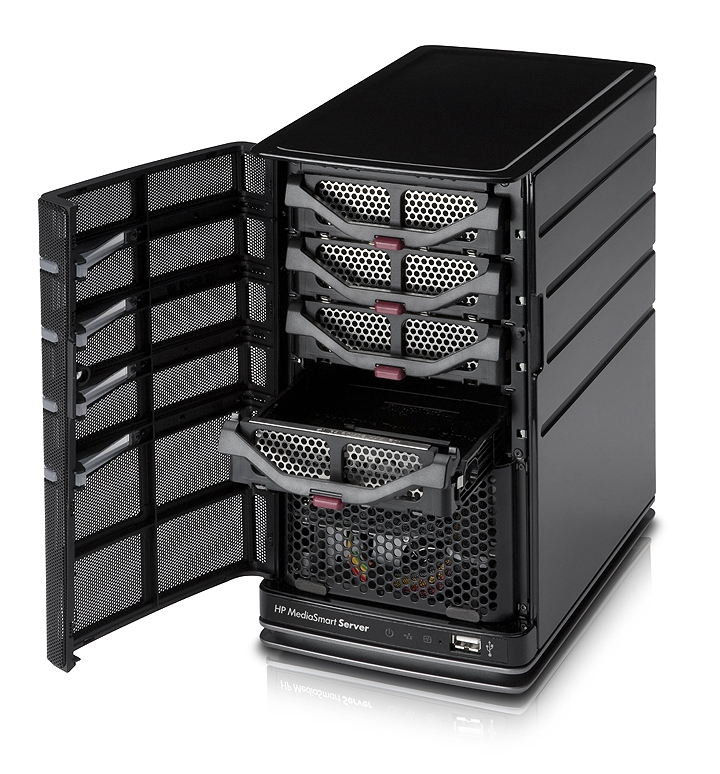
\includegraphics[scale=0.17]{img/hp-server.jpg}
      \end{figure}
    \end{column}
    \pause
    \begin{column}[l]{0.45\textwidth}
      \begin{center}
        What to do?
      \end{center}
      \begin{figure}
         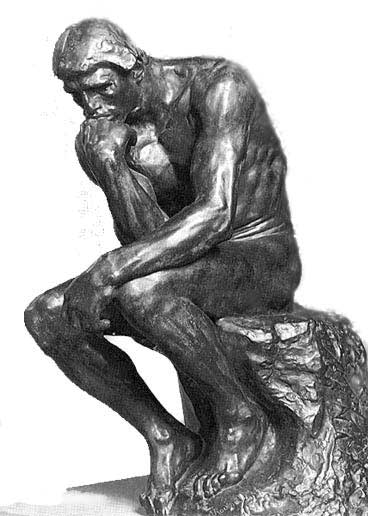
\includegraphics[scale=0.25]{img/thinker.jpg}
      \end{figure}
    \end{column}
  \end{columns}
\end{frame}

\begin{frame}[fragile]{Verbatim text}
  \pause
  \footnotesize
  \begin{verbatim}
brw-rw----  1 root disk      8,   0 Oct  2 21:53 sda
brw-rw----  1 root disk      8,   1 Oct  2 21:53 sda1
brw-rw----  1 root disk      8,  10 Oct  2 18:53 sda10
brw-rw----  1 root disk      8,  11 Oct  2 21:53 sda11
crw-rw----  1 root root      4,   0 Oct  2 21:53 tty0
crw-rw----  1 root root      4,  10 Oct  2 21:53 tty10
crw-rw----  1 root root      4,  11 Oct  2 21:53 tty11
crw-rw----  1 root root      4,  12 Oct  2 21:53 tty12
  \end{verbatim}
\end{frame}

\section{Keywords}

\begin{frame}{Keywords}
  \begin{columns}
    \begin{column}[l]{0.5\textwidth}
      \begin{itemize}
        \item research
        \item papers
      \end{itemize}
    \end{column}
    \begin{column}[l]{0.5\textwidth}
      \begin{itemize}
        \item group
        \item conference
      \end{itemize}
    \end{column}
  \end{columns}
\end{frame}

\begin{frame}{Other resources}
  \begin{itemize}
    \item James Turnbull, Peter Lieverdink, Dennis Matotek -- Pro Linux System
    Administration
    \item \url{http://elf.cs.pub.ro/pisr/}
    \item
    \url{http://www.lpi.org/index.php/eng/certification/the_lpic_program}
    \item \url{http://debian.org/doc/user-manuals}
    \item \url{http://wiki.debian.org/}
    \item \url{http://www.debian-administration.org/}
  \end{itemize}
\end{frame}

\section{Questions}

\end{document}
